\section{Pose Graph Optimization}

When the amount of registered captures increment, the accumulated error 
becomes more visible. There is a drift respect to the real sensor trajectory. 
In order to afront this problem the most common approach is to use a pose graph 
optimization algorithm. 

Each pose of the sensor (rotation and translation) represents a node of the 
graph and each restriction between two poses represents an edge. The relative 
transformation between the two poses is used as restriction and it is possible 
to add different kinds of restrictions if more information is available.

Then we have a least squares minimization problem that can be described by the following equation:

$$ F(x) = \sum\limits_{<i,j> \in C } e(x_i,x_j,z_{ij})^T \Omega_{ij} e(x_i,x_j,z_{ij}) $$

$$ x^* = \mathop{\rm argmin}_x F(x) $$

Where $x=\{x_1,x_2,...,x_n\}$ and each $x_i$ represents a parameter block , $z_{i,j}$ and $\Omega_{ij}$ represents the mean  
 and the information matrix  of a constraint 
relating parameters $x_i$ and $x_j$.

Poses and relative transformations are represented by a 7x1 vector containing a quaternion $(qx,qy,qz,qw)$ 
for the rotation and a traslation vector $(tx,ty,tz)$.

In our case $x_i$ corresponds to a sensor pose, $z_{i,j}$ is the 
relative transformation between the pose i-esim and j-esim sensor capture, it is not affected by the accumulated error 
because it is a direct measure between the two captures and $\Omega_{ij}$ is the weight or 
the confidence we give to the restriction. $\Omega_{ij}$ is a 7x7 diagonal matrix, containg on its diagonal the confidence for each 
parameter of the transformation.

This is a non linear least squares problem and can be solved using 
methods such as for example Gauss-Newton or Levenber-Marquardt.


then $e_{ij}$ is defined as follows:

$$
e(x_i,x_j,z_{ij}) = z_{ij} - \hat{z_{ij}}
$$

Where $\hat{z_{ij}}$ is the relative transformation obtained directly from the pose graph, for this reason 
it is affected by the accumulated error.

We want to find a graph configuration (updating the poses $x=\{x_1,x_2,...,x_n\}$), in order to reduce 
the global error, correcting some poses in order to satisfy the restrictions.

To simplify notation let 

$$
e(x_i,x_j,z_{ij}) = e(x_i,x_j) = e_{ij}(x)
$$

We can approximate the previous function around one point:

\begin{equation}
\label{eq:errorAprox}
e_{ij}(x + \Delta x) \simeq e_{ij}(x) + J_{ij} \Delta x
\end{equation}

$J_{ij}$ is the Jacobian of the function evaluated in x. 


\begin{equation}
\label{eq:globalFunc}
F_{ij}(x + \Delta x) = e_{ij}(x + \Delta x)^T \Omega_{ij}  e_{ij}(x + \Delta x)
\end{equation}

Reeplacing \ref{eq:errorAprox} in the global function:

\begin{equation}
\label{eq:globalFuncAprox}
F_{ij}(x + \Delta x) \simeq (e_{ij}(x) + J_{ij} \Delta x)^T \Omega_{ij}  (e_{ij}(x) + J_{ij} \Delta x)
\end{equation}

\begin{equation}
\label{eq:globalFuncAprox2}
 =  \underbrace{e_{ij}(x)^T \Omega_{ij} e_{ij}(x)}_{c_{ij}} + 2  \underbrace{e_{ij}(x)^T \Omega_{ij} J_{ij}}_{b_{ij}} \Delta x + \Delta x^T \underbrace{ J_{ij}^T  \Omega_{ij} J_{ij}}_{H_{ij}} \Delta x
\end{equation}

\begin{equation}
\label{eq:globalFuncAprox2}
 = c_{ij} + 2 b_{ij} \Delta x + \Delta x^T H_{ij} \Delta x
\end{equation}


\begin{equation}
F(x + \Delta x) =  \sum\limits_{<i,j> \in C } F_{ij}(x + \Delta x) 
\end{equation}



\begin{equation}
\simeq  c_{ij} + 2 b_{ij} \Delta x + \Delta x^T H_{ij} \Delta x
=   c + 2 b \Delta x + \Delta x^T H \Delta x
\end{equation}

Then we want to know $\Delta x^T$, this is the correction to the $x_i$ and $x_j$ nodes, in order 
to have a minimum error:

\begin{equation}
H \Delta x^* = -b
\end{equation}

Having $\Delta x^T$ we can update the graph nodes:

\begin{equation}
x^* = x + \Delta x^* 
\end{equation}

This is the Gauss-Newton algorithm. 

The Levenber-Marquardt (LM) is a nonlinear variant of the Gauss-Newton algorithm that introduces a
damping factor and backup actions to control the convergence:

\begin{equation}
(H + \lambda I) \Delta x^* = -b
\end{equation}

The $\lambda$ factor controls the size of $ \Delta x$. Allowing to change it according to the error between the iterations.
 


G2o is a library that contains non linear error functions optimization 
algorithms for graphs and is widely used in registration algorithms. 

The poses where optimized using this library and specifically the 
Levenber-Marquardt algorithm.

In the thesis the following definition for $z_{ij}$ was used:

\begin{equation}
z_{ij} = [tx ty tz qx qy qz qw]
\end{equation}

Where (tx,ty,tz) is a translation vector and (qx,qy,qz,qw) is a quaternion.

\subsection{Loop Closure}

When the sensor vists the same region at different times, for example following 
a circular trajectory. A restriction between two non-consecutive captures can be 
added to the graph. In the case of a circular trajectory, the accumulated error 
is very noticeable when the initial and the final capture are connected. If a 
restriction between this two captures is added to the graph it is possible to 
adjust the position of all poses in order to satisfy the restriction. This 
is called Loop Closure.


\begin{figure}[!h]
\begin{center}
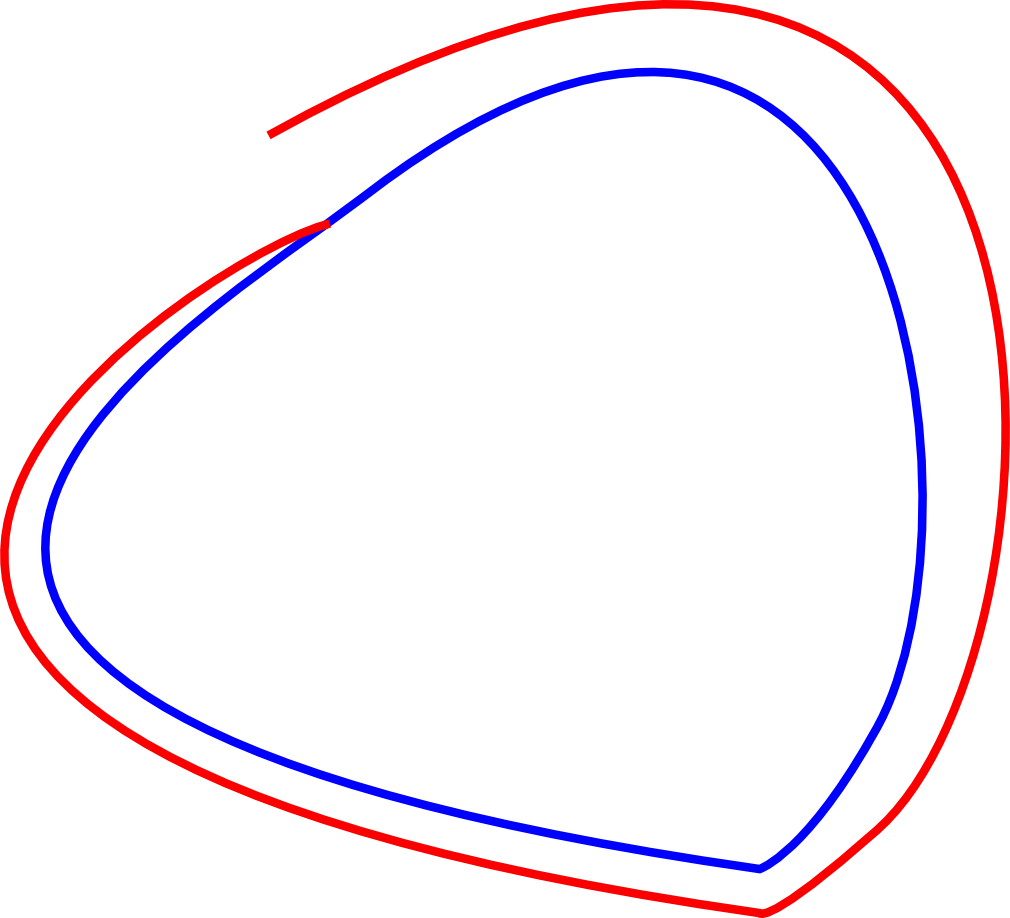
\includegraphics[scale=0.35]{images/drift}
\caption{Example of drift from real trajectory. Blue color: real camera trajectory, red color: estimation of trajectory with accumulated error.}
\end{center}
\end{figure}

\subsection{Loop Detection}

In order to detect previously visited areas of the scene SURF \cite{Bay06surf} feature detector 
is used. 

